\documentclass[12pt,a4paper]{article}

% ─── Page Layout ───────────────────────────────────────────────────────────────
\usepackage[a4paper, margin=0.8in, headheight=14pt]{geometry}

% ─── Fonts (XeLaTeX) ───────────────────────────────────────────────────────────
\usepackage{fontspec}
\usepackage{unicode-math}
\setmainfont{TeX Gyre Pagella}
\setmonofont[Scale=0.88]{TeX Gyre Cursor}
\setmathfont{Latin Modern Math}

% ─── Packages ──────────────────────────────────────────────────────────────────
\usepackage{xcolor}
\usepackage{colortbl}
\usepackage{titlesec}
\usepackage{enumitem}
\usepackage{tabularx}
\usepackage{booktabs}
\usepackage{array}
\usepackage{amsmath}
\usepackage{tikz}
\usetikzlibrary{shapes.geometric, arrows.meta, positioning, calc, fit, decorations.pathreplacing, patterns}
\usepackage{tcolorbox}
\tcbuselibrary{skins, breakable}
\usepackage{hyperref}
\usepackage{fancyhdr}
\usepackage{graphicx}
\usepackage{microtype}
\hyphenpenalty=10000
\exhyphenpenalty=10000
\sloppy
\usepackage{caption}
\usepackage{setspace}
\usepackage{multirow}
\usepackage{tocloft}

% ─── Q&A helper ────────────────────────────────────────────────────────────────
\newcommand{\Q}[1]{\textbf{#1}\par\noindent\ignorespaces}

% ─── Colour Palette ────────────────────────────────────────────────────────────
\definecolor{myred}{RGB}{196,30,58}
\definecolor{mydark}{RGB}{30,30,50}
\definecolor{mygreen}{RGB}{14,120,80}
\definecolor{myteal}{RGB}{0,130,140}
\definecolor{myamber}{RGB}{180,100,0}
\definecolor{mypurple}{RGB}{100,30,160}
\definecolor{mygray}{RGB}{246,247,249}
\definecolor{mgframe}{RGB}{180,185,200}
\definecolor{watermark}{RGB}{145,150,170}
\definecolor{hdrred}{RGB}{250,232,235}
\definecolor{hdrgreen}{RGB}{220,244,233}
\definecolor{hdrteal}{RGB}{220,242,244}
\definecolor{hdramber}{RGB}{253,242,215}
\definecolor{hdrpurple}{RGB}{238,228,255}
\definecolor{hdrgray}{RGB}{238,240,245}
\definecolor{rowalt}{RGB}{250,251,253}

% ─── Section Formatting ────────────────────────────────────────────────────────
\titleformat{\section}{\large\bfseries\color{myred}}{\thesection.}{0.5em}{}[\vspace{1pt}{\color{myred}\rule{\linewidth}{0.8pt}}]
\titleformat{\subsection}{\normalsize\bfseries\color{myteal}}{\thesubsection}{0.5em}{}
\titlespacing*{\section}{0pt}{18pt}{7pt}
\titlespacing*{\subsection}{0pt}{11pt}{4pt}

% ─── Paragraph ─────────────────────────────────────────────────────────────────
\setlength{\parindent}{0pt}
\setlength{\parskip}{4pt}

% ─── TOC Styling ───────────────────────────────────────────────────────────────
\renewcommand{\cfttoctitlefont}{\large\bfseries\color{myred}}
\renewcommand{\cftaftertoctitle}{\par\noindent{\color{myred}\rule{\linewidth}{0.8pt}}}
\setlength{\cftbeforetoctitleskip}{0pt}
\setlength{\cftaftertoctitleskip}{6pt}
\renewcommand{\cftsecfont}{\normalsize\bfseries\color{mydark}}
\renewcommand{\cftsecpagefont}{\normalsize\bfseries\color{mydark}}
\renewcommand{\cftsecleader}{\cftdotfill{\cftdotsep}}
\setlength{\cftbeforesecskip}{7pt}
\renewcommand{\cftsubsecfont}{\small\color{mydark}}
\renewcommand{\cftsubsecpagefont}{\small\color{mydark}}
\setlength{\cftbeforesubsecskip}{3pt}
\setlength{\cftsubsecindent}{1.4em}

% ─── Table helpers ─────────────────────────────────────────────────────────────
\renewcommand{\arraystretch}{1.45}
\setlength{\tabcolsep}{6pt}
\arrayrulecolor{mydark}
\newcolumntype{B}[1]{>{\small\bfseries\raggedright\arraybackslash}m{#1}}
\newcolumntype{Y}{>{\small\raggedright\arraybackslash}X}
\renewcommand{\tabularxcolumn}[1]{m{#1}}

% ─── Header / Footer ───────────────────────────────────────────────────────────
\pagestyle{fancy}
\fancyhf{}
\fancyhead[L]{\small\color{myred}\textbf{OE-EC803B}\;\color{mydark}--- Big Data Analysis}
\fancyhead[R]{\small\color{myteal}\textbf{Module 2 Notes}}
\fancyfoot[C]{\small\color{mydark}\thepage}
\fancyfoot[R]{\small\color{watermark}\textit{\copyright\ Biraj Sarkar}}
\renewcommand{\headrulewidth}{0.5pt}
\renewcommand{\footrulewidth}{0.3pt}

% ─── Hyperref ──────────────────────────────────────────────────────────────────
\hypersetup{colorlinks=true, linkcolor=myteal, urlcolor=myteal,
  pdfauthor={Biraj Sarkar}, pdftitle={OE-EC803B --- Module 2 Notes}}

% ─── tcolorbox styles ──────────────────────────────────────────────────────────
\tcbset{
  tikzbox/.style={colback=mygray, colframe=mgframe, boxrule=0.6pt, arc=4pt,
    left=8pt, right=8pt, top=6pt, bottom=6pt,
    colbacktitle=mgframe, coltitle=mydark, fonttitle=\small\bfseries, unbreakable},
  defbox/.style={colback=hdrgreen, colframe=mygreen, boxrule=0.8pt, arc=4pt,
    left=9pt, right=9pt, top=6pt, bottom=6pt,
    colbacktitle=mygreen, coltitle=white, fonttitle=\small\bfseries},
  formulabox/.style={colback=hdrteal, colframe=myteal, boxrule=0.8pt, arc=4pt,
    left=9pt, right=9pt, top=7pt, bottom=7pt,
    colbacktitle=myteal, coltitle=white, fonttitle=\small\bfseries},
  examplebox/.style={colback=hdramber, colframe=myamber, boxrule=0.8pt, arc=4pt,
    left=9pt, right=9pt, top=6pt, bottom=6pt,
    colbacktitle=myamber, coltitle=white, fonttitle=\small\bfseries},
  masonbox/.style={colback=hdrpurple, colframe=mypurple, boxrule=0.8pt, arc=4pt,
    left=9pt, right=9pt, top=6pt, bottom=6pt,
    colbacktitle=mypurple, coltitle=white, fonttitle=\small\bfseries},
  exambox/.style={colback=hdrpurple, colframe=mypurple, boxrule=1pt, arc=5pt,
    left=10pt, right=10pt, top=8pt, bottom=8pt,
    colbacktitle=mypurple, coltitle=white, fonttitle=\bfseries,
    breakable, title after break={\textbf{Frequently Asked / Viva Questions (contd.)}}}
}
\tcbset{breakable}

% ─── TikZ styles ───────────────────────────────────────────────────────────────
\tikzset{
  block/.style={rectangle, draw=myteal, fill=hdrteal,
    text width=2.2cm, align=center, minimum height=0.9cm,
    font=\small, rounded corners=3pt, line width=0.7pt},
  redblock/.style={rectangle, draw=myred, fill=hdrred,
    text width=2.2cm, align=center, minimum height=0.9cm,
    font=\small, rounded corners=3pt, line width=0.7pt},
  arrow/.style={-Stealth, thick, color=mydark},
  redarrow/.style={-Stealth, thick, color=myred},
  line/.style={thick, color=mydark}
}

\begin{document}

% ═══════════════════════════════════════════════════════════════════════════════
% TITLE BLOCK
% ═══════════════════════════════════════════════════════════════════════════════
\begin{center}
  \hfill \textit{Exam-Ready Short Notes} \\
  \vspace{6pt}
  {\LARGE\bfseries\color{myred} OE-EC803B --- Big Data Analysis}\\[5pt]
  {\normalsize\color{mydark} Semester VIII \quad$\bullet$\quad 3L:0T:0P \quad$\bullet$\quad 3 Credits}\\[3pt]
  {\normalsize\color{myteal}\textbf{Module 2: HDFS (Hadoop Distributed File System) \& I/O}}\\[3pt]
  {\small\color{mydark} CGEC \;$|$\; B.Tech ECE (2023--27) \;$|$\; \textit{Biraj Sarkar}}
\end{center}
\vspace{2pt}
\noindent{\color{myred}\rule{\linewidth}{1.5pt}}
\vspace{2pt}

\hypersetup{linkcolor=mydark}
\tableofcontents
\hypersetup{linkcolor=myteal}
\newpage

% ===============================================================================
\section{The Design of HDFS}
% ===============================================================================

\begin{tcolorbox}[defbox, title={Hadoop Distributed File System (HDFS)}]
  \textbf{HDFS} is a distributed, block-structured file system designed to store very large files (typically Gigabytes to Petabytes) reliably across a cluster of commodity servers, providing high throughput access to application data using a write-once, read-many access pattern.
\end{tcolorbox}

Key design goals and assumptions include:
\begin{itemize}[leftmargin=*, itemsep=3pt]
  \item \textbf{Commodity Hardware Failure:} HDFS assumes hardware failures are common rather than exceptional. High fault tolerance is built in through automatic block replication.
  \item \textbf{Large Datasets:} Optimized to support large files. A single HDFS cluster can support millions of files.
  \item \textbf{Streaming Data Access:} Designed for batch processing rather than low-latency interactive access. Focuses on high data throughput over low latency.
  \item \textbf{Simple Coherency Model:} Uses a \textbf{write-once, read-many} pattern. Once a file is written, closed, and replicated, it cannot be modified inline. Appends are supported in later versions but random edits are not.
\end{itemize}

% ===============================================================================
\section{HDFS Concepts}
% ===============================================================================

\subsection{Blocks in HDFS}
Unlike standard physical hard drives where disk blocks are 512 bytes or 4KB, HDFS files are divided into large, discrete chunks called \textbf{Blocks}.

\begin{tcolorbox}[formulabox, title={HDFS Block Size Properties}]
  The standard block size in modern Hadoop distributions is \textbf{128MB} (or \textbf{256MB}).
  \begin{itemize}[leftmargin=*, noitemsep]
    \item \textbf{Reason for large blocks:} To minimize the cost of disk seeks. By making blocks large, the time taken to transfer data from disk to network is significantly larger than the time taken to seek to the start of the block.
    \item \textbf{Block Storage:} If a file is smaller than the block size (e.g., a 10MB file), it does not consume the full 128MB of physical space; it only uses 10MB on the local disk.
  \end{itemize}
\end{tcolorbox}

\subsection{NameNode, DataNode, and Secondary NameNode}
HDFS uses a master-slave architecture containing three key operational nodes:

\begin{tcolorbox}[tikzbox, title={HDFS Master-Slave Architecture}]
\centering
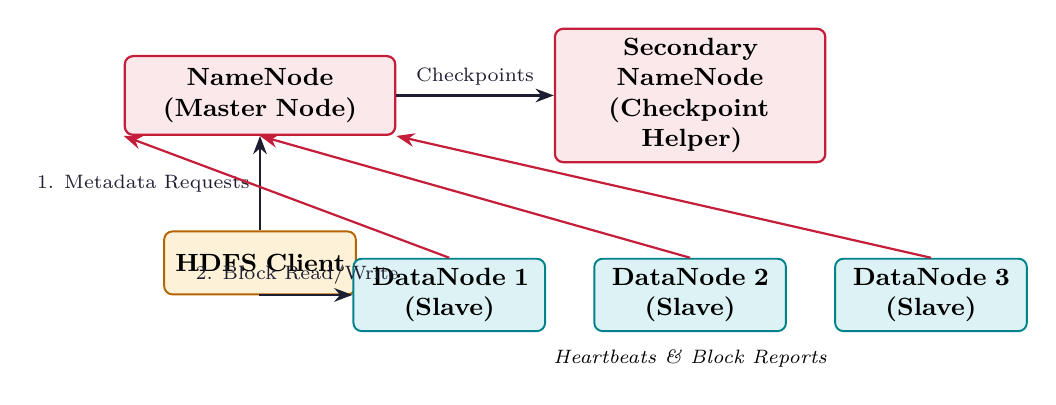
\begin{tikzpicture}[node distance=1.0cm and 1.5cm,
  mnode/.style={rectangle, draw=myred, fill=hdrred, text width=3.2cm, align=center, minimum height=1.0cm, font=\small\bfseries, rounded corners=3pt, line width=0.8pt},
  snode/.style={rectangle, draw=myteal, fill=hdrteal, text width=2.2cm, align=center, minimum height=0.9cm, font=\small\bfseries, rounded corners=3pt, line width=0.7pt},
  cnode/.style={rectangle, draw=myamber, fill=hdramber, text width=2.2cm, align=center, minimum height=0.8cm, font=\small\bfseries, rounded corners=3pt, line width=0.7pt}]

  % Nodes
  \node[mnode] (nn) {NameNode\\(Master Node)};
  \node[mnode, right=2.0cm of nn] (snn) {Secondary NameNode\\(Checkpoint Helper)};
  \node[cnode, below=1.2cm of nn] (client) {HDFS Client};

  \node[snode, below=1.2cm of snn] (dn2) {DataNode 2\\(Slave)};
  \node[snode, left=0.6cm of dn2] (dn1) {DataNode 1\\(Slave)};
  \node[snode, right=0.6cm of dn2] (dn3) {DataNode 3\\(Slave)};

  % Arrows
  \draw[arrow] (client) -- node[left, font=\scriptsize] {1. Metadata Requests} (nn);
  \draw[arrow] (client) |- node[pos=0.7, above, font=\scriptsize] {2. Block Read/Write} (dn1.west);
  \draw[arrow] (nn) -- node[above, font=\scriptsize] {Checkpoints} (snn);

  \draw[redarrow] (dn1.north) -- (nn.south west);
  \draw[redarrow] (dn2.north) -- (nn.south);
  \draw[redarrow] (dn3.north) -- (nn.south east);

  % Correct formatting for node text next to diagram
  \node[below=0.1cm of dn2, font=\scriptsize\itshape] {Heartbeats \& Block Reports};

\end{tikzpicture}
\end{tcolorbox}

\begin{itemize}[leftmargin=*, itemsep=4pt]
  \item \textbf{NameNode (Master):}
    \begin{itemize}[noitemsep]
      \item Manages the file system namespace (directories, files).
      \item Tracks the mapping of files to block IDs and their physical DataNode locations.
      \item Stores metadata in RAM for speed. Persists namespace changes in the \textbf{Edit Log} and holds the point-in-time filesystem state in \textbf{FSImage}.
    \end{itemize}
  \item \textbf{DataNode (Slave):}
    \begin{itemize}[noitemsep]
      \item Stores and retrieves HDFS data blocks on the local physical filesystem as directed by the NameNode.
      \item Sends periodic \textbf{Heartbeats} (confirming node availability) and \textbf{Block Reports} (listing all local blocks) to the NameNode.
    \end{itemize}
  \item \textbf{Secondary NameNode:}
    \begin{itemize}[noitemsep]
      \item It is NOT a backup/failover NameNode.
      \item It periodically merges the active \textbf{Edit Log} with the \textbf{FSImage} to prevent the Edit Log from growing too large. This process is called \textbf{Checkpointing}.
    \end{itemize}
\end{itemize}

% ===============================================================================
\section{HDFS Interfaces and Command Line Interface}
% ===============================================================================

\subsection{HDFS CLI (Command Line Interface)}
Users interact with HDFS files using standard terminal commands prefixed with `hdfs dfs` or `hadoop fs`.

\begin{tcolorbox}[examplebox, title={Common HDFS Terminal Commands}]
\renewcommand{\arraystretch}{1.3}
\begin{tabularx}{\linewidth}{|B{3.5cm}|Y|}
\hline
\textbf{Command} & \textbf{Description and Syntax} \\
\hline
`hdfs dfs -ls <path>` & Lists directory contents (analogous to Unix `ls`). \\
\hline
`hdfs dfs -put <src> <dest>` & Copies a local file from the client host into HDFS. \\
\hline
`hdfs dfs -get <src> <dest>` & Retrieves a file from HDFS and stores it locally. \\
\hline
`hdfs dfs -cat <path>` & Displays file contents directly on stdout. \\
\hline
`hdfs dfs -mkdir <path>` & Creates a new directory in HDFS. \\
\hline
`hdfs dfs -rm <path>` & Deletes a file or folder from HDFS. \\
\hline
\end{tabularx}
\end{tcolorbox}

\subsection{Hadoop File System Interfaces}
Hadoop supports programmatic interfaces to access HDFS files:
\begin{enumerate}[leftmargin=*, itemsep=3pt]
  \item \textbf{Java API:} The native interface. Uses the `org.apache.hadoop.fs.FileSystem` abstraction class, executing methods like `open()`, `create()`, and `delete()`.
  \item \textbf{WebHDFS REST API:} Provides complete read/write HTTP REST protocol endpoints to interact with HDFS from non-Java languages without loading fat native client libraries.
\end{enumerate}

% ===============================================================================
\section{HDFS Data Flow}
% ===============================================================================

Data flow operations in HDFS isolate the client from the details of block replication and network routing.

\subsection{Anatomy of a File Read}
\begin{enumerate}[leftmargin=*, itemsep=3pt]
  \item The Client calls `open()` on the `FileSystem` object (which is a `DistributedFileSystem` instance).
  \item The `DistributedFileSystem` calls the NameNode using RPC (Remote Procedure Call) to get the locations of the blocks for the first part of the file.
  \item The NameNode returns a list of DataNodes that have copies of those blocks, sorted by network proximity to the client.
  \item The client calls `read()` on the input stream (`FSDataInputStream`), which connects to the nearest DataNode.
  \item Once the end of the block is reached, `FSDataInputStream` closes the connection to that DataNode and opens a connection to the nearest DataNode for the next block, until reading is complete.
\end{enumerate}

\subsection{Anatomy of a File Write}
\begin{enumerate}[leftmargin=*, itemsep=3pt]
  \item The Client calls `create()` on the `DistributedFileSystem` object.
  \item The `DistributedFileSystem` makes an RPC call to the NameNode to create a new file in the filesystem namespace. The NameNode checks permissions and verifies the path does not already exist.
  \item The client writes data to the output stream (`FSDataOutputStream`), which splits it into packets and writes them to an internal queue called the \textbf{Data Queue}.
  \item The \textbf{Data Streamer} requests the NameNode to allocate new blocks and choose DataNodes to store replicas (typically 3 DataNodes for a replication factor of 3).
  \item A pipeline is formed between the selected DataNodes (e.g., DataNode A $\rightarrow$ DataNode B $\rightarrow$ DataNode C). The Data Streamer streams packets to the first DataNode, which passes them to the second, which passes them to the third.
  \item When the client finishes writing data, it calls `close()`, which flushes all remaining packets to the DataNodes and contacts the NameNode to commit the file creation.
\end{enumerate}

% ===============================================================================
\section{Data Ingestion: Sqoop and Flume}
% ===============================================================================

To analyze data in Hadoop, it must first be ingested from external sources.

\subsection{Apache Sqoop}
\begin{tcolorbox}[defbox, title={Apache Sqoop (SQL to Hadoop)}]
  \textbf{Sqoop} is a tool designed to transfer bulk data between relational databases (RDBMS) and the Hadoop Ecosystem (HDFS, Hive, HBase). It translates import and export commands into MapReduce jobs to execute parallel data transfers.
\end{tcolorbox}

\begin{itemize}[leftmargin=*, itemsep=3pt]
  \item \textbf{Import Mechanism:} Reads rows from an RDBMS table, generates a MapReduce job where mappers read data in parallel using SQL boundaries, and writes the output files to HDFS.
  \item \textbf{Export Mechanism:} Reads files from HDFS and inserts records into a target database table in parallel using database insert statements.
\end{itemize}

\subsection{Apache Flume}
\begin{tcolorbox}[defbox, title={Apache Flume}]
  \textbf{Flume} is a distributed service designed for efficiently collecting, aggregating, and moving large amounts of streaming log data (such as web server logs or social media streams) into HDFS.
\end{tcolorbox}

An active Flume agent consists of three main components:
\begin{enumerate}[leftmargin=*, itemsep=3pt]
  \item \textbf{Source:} Receives event data from external generators (e.g., Syslog, HTTP) and pushes it into one or more channels.
  \item \textbf{Channel:} A passive store that buffers the events until they are consumed by a sink (can be in-memory for speed or file-based for durability).
  \item \textbf{Sink:} Removes events from the channel and stores them in an external repository like HDFS or HBase.
\end{enumerate}

% ===============================================================================
\section{Hadoop Archives (HAR)}
% ===============================================================================

Every file, directory, and block in HDFS occupies about 150 bytes of memory in the NameNode's RAM. If a cluster stores millions of small files (smaller than the block size), the NameNode RAM becomes a performance bottleneck.

\begin{tcolorbox}[defbox, title={Hadoop Archives (HAR)}]
  \textbf{Hadoop Archives (HAR)} are file archiving tools that pack HDFS files into larger archive files (`.har` files) to reduce the metadata overhead in the NameNode, while still allowing applications to access the individual files transparently.
\\
A `.har` archive contains index files listing the metadata and a set of part files containing the concatenated data blocks.
\end{tcolorbox}

% ===============================================================================
\section{Hadoop I/O: Compression, Serialization, and File Structures}
% ===============================================================================

\subsection{Compression Codecs}
Hadoop supports data compression to save storage space and reduce network and disk I/O overhead.

\par\vspace{6pt}\noindent
{\renewcommand{\arraystretch}{1.4}%
\begin{tabularx}{\linewidth}{|B{2.5cm}|Y|Y|Y|}
\hline
\textbf{Codec} & \textbf{Algorithm} & \textbf{Splittable?} & \textbf{Key Characteristics} \\
\hline
\textbf{Gzip} & DEFLATE & No & High compression ratio, slow speed. \\
\hline
\textbf{Bzip2} & Burrows-Wheeler & Yes & Extremely high compression ratio, very slow. \\
\hline
\textbf{LZO} & LZO & Yes (if indexed) & Fast compression and decompression. \\
\hline
\textbf{Snappy} & Snappy & No & Very fast speed, moderate compression. \\
\hline
\end{tabularx}}

\textbf{Why Splittability Matters:} If a compression format is splittable, MapReduce can split the file and process different portions on separate mappers in parallel. If it is not splittable, a single mapper must process the entire file sequentially, breaking the parallel execution model.

\subsection{Serialization}
\begin{tcolorbox}[defbox, title={Serialization}]
  \textbf{Serialization} is the process of converting structured objects into a stream of bytes for transmission over a network or storage on disk. \textbf{Deserialization} is the reverse process of turning a byte stream back into live runtime objects.
\end{tcolorbox}

Hadoop does not use standard Java serialization because it is too bloated. Instead, it defines its own lightweight protocols:
\begin{itemize}[leftmargin=*, itemsep=3pt]
  \item \textbf{Writable Interface:} Mappers and Reducers exchange keys and values implementing the \textbf{Writable} interface. It provides high-speed serialization using compact byte formats.
  \item \textbf{Avro:} A language-neutral serialization system that stores data schemas in JSON files, making it easy for different languages (Java, C++, Python) to share data records.
\end{itemize}

\subsection{File-Based Data Structures}
Hadoop provides specialized container files for binary data:
1. \textbf{SequenceFile:} A persistent, binary container file format for storing key-value pairs. It supports compression and includes \textbf{sync markers} to allow MapReduce splits.
2. \textbf{MapFile:} A sorted version of \textbf{SequenceFile} that contains an index file (`/index`) alongside the data file (`/data`) to allow fast random access by key.

\newpage

% ═══════════════════════════════════════════════════════════════════════════════
% QUICK REVISION PAGE
% ═══════════════════════════════════════════════════════════════════════════════
\begin{center}
  {\large\bfseries\color{myred} Quick Revision --- Module 2}\\[3pt]
  {\small\color{mydark} HDFS Concepts, CLI \& I/O Architectures $|$ OE-EC803B}
\end{center}
\noindent{\color{myred}\rule{\linewidth}{1.2pt}}
\vspace{8pt}

\begin{tcolorbox}[defbox, title={\textbf{One-Line Definitions}}]
\begin{itemize}[leftmargin=*, itemsep=3pt, topsep=0pt]
  \item \textbf{DataNode:} A slave node in HDFS that physically stores data blocks on local disks.
  \item \textbf{Secondary NameNode:} A helper node that periodically merges Edit Logs with FSImage (Checkpointing).
  \item \textbf{Splittability:} The property of a file format/codec that allows it to be split into chunks for parallel MapReduce execution.
  \item \textbf{SequenceFile:} A persistent binary file format that stores sequential key-value data.
  \item \textbf{Avro:} A serialization framework using JSON-defined schemas for cross-language data exchanges.
\end{itemize}
\end{tcolorbox}

\vspace{6pt}

\begin{tcolorbox}[exambox, title={\textbf{Frequently Asked / Viva Questions}}]
\begin{enumerate}[leftmargin=*, topsep=0pt, label=\textbf{Q\arabic*.}, itemsep=5pt]
  \item \Q{Why does HDFS use a large block size (e.g., 128MB)?}
        Large block sizes minimize the disk seek overhead. Since disk seeks take several milliseconds, setting the block size to 128MB ensures that the disk transfer time (reading data) is significantly larger than the seek time, maximizing throughput.
        
  \item \Q{How does checkpointing work in the Secondary NameNode?}
        The Secondary NameNode fetches the active Edit Log and current FSImage from the NameNode, merges them in memory to generate a new FSImage checkpoint, and sends it back to the NameNode. This keeps the Edit Log from growing too large.
        
  \item \Q{Describe the HDFS replication strategy (Rack Awareness).}
        For a replication factor of 3: HDFS places the first replica on a node in the local rack, the second replica on a different node in a remote rack, and the third replica on a different node within that same remote rack. This balances fault tolerance and write latency.
        
  \item \Q{What happens if a DataNode fails in an HDFS cluster?}
        If a DataNode fails to send Heartbeats to the NameNode for a timeout period (typically 10 minutes), the NameNode marks it as dead. It scans the metadata, identifies all blocks stored on the failed node, and schedules copies of those blocks to other nodes to restore the replication factor.
        
  \item \Q{What is the difference between client-side reads and client-side writes in HDFS?}
        During a read, the client only queries the NameNode for block locations and reads directly from the nearest DataNode. During a write, the client streams packets to a pipeline of DataNodes, which replicate data to each other while sending ACKs back.
        
  \item \Q{Explain the agent architecture of Apache Flume.}
        A Flume agent consists of a \textbf{Source} (ingests raw logs from external clients), a \textbf{Channel} (buffers events in memory or on disk), and a \textbf{Sink} (drains the channel to write files into HDFS).
        
  \item \Q{Why are Hadoop Archives (HAR) used for small files?}
        Each file in HDFS consumes 150 bytes of metadata in the NameNode's RAM. Millions of small files can exhaust NameNode memory. HAR bundles these files into larger archive containers, reducing the total metadata footprint.
        
  \item \Q{Which compression codecs are splittable in MapReduce?}
        Bzip2 is natively splittable. LZO is splittable if an index is built for it. Gzip and Snappy are not splittable.
        
  \item \Q{Why did Hadoop develop its own Writable serialization system instead of using Java Serialization?}
        Java's default serialization is too heavy, storing class names, parent classes, and metadata along with the data. Hadoop's Writable system is lightweight, compact, and optimized for high-speed network transmission.
        
  \item \Q{What is the difference between a SequenceFile and a MapFile?}
        A SequenceFile stores binary key-value pairs sequentially. A MapFile is a directory containing a sorted SequenceFile (`/data`) and an index file (`/index`) that maps keys to offsets for random lookups.
\end{enumerate}
\end{tcolorbox}

\vspace{6pt}

\begin{tcolorbox}[tikzbox, title={\textbf{Comparison Snapshot}}]
\textbf{NameNode vs. DataNode:}\par\vspace{6pt}\noindent
{\renewcommand{\arraystretch}{1.4}%
\begin{tabularx}{\linewidth}{|B{3.2cm}|Y|Y|}
\hline
\textbf{Feature} & \textbf{NameNode} & \textbf{DataNode} \\
\hline
Role & Master Node & Slave Node \\
\hline
Primary Data stored & File metadata, namespace mapping, block locations & Actual data blocks (replicated payload) \\
\hline
Storage Media & System RAM (for speed) & Physical Hard Drive / SSD \\
\hline
Hardware requirements & Enterprise grade (high RAM capacity) & Commodity servers (large storage disks) \\
\hline
Quantity in Cluster & Active/Standby pair (HA configurations) & Thousands of nodes in large clusters \\
\hline
Failure Impact & High (cluster down if master fails without HA) & Low (re-replicated from other nodes) \\
\hline
\end{tabularx}}
\end{tcolorbox}

\end{document}
